\chapter{Background}
\label{ch:background}

This chapter explains the fundamental topics required to understand this thesis.

\section{Knowledge Graph} 
\label{sec:knowledge_graph}
Knowledge Graphs are graphs intended to represent knowledge of the real world or smaller scenarios.
The knowledge stored in Knowledge Graphs is modeled in a graph-based structure. 
Nodes represent entities which are connected by various types of relations, represented by labeled edges in the graph.
This has the benefit to represent complex relations between different nodes and edges\cite{hoganKnowledgeGraphs2021}.

The simplest knowledge graph consists of three elements.
The subject entity, the object entity and the labeled edge between them describing their relation.
This atomic data entity is called triple.

In figure \ref{fig:example-knowledge-graph} a simple example of a knowledge graph is shown.

\begin{figure}[tbph]
	\centering
	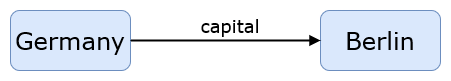
\includegraphics[width=0.4\textwidth]{figures/knowledge-graph-diagram}
	\caption{Simple Knowledge Graph}
	\label{fig:example-knowledge-graph}
\end{figure}

Since a graph structure is hard to store in a classic relational database a different type of storage is needed.
The special kind of database developed to store knowledge graphs are called \tsp{}.


\section{\ts{}}
\label{sec:triplestores}
\tsp{} are a special kind of database developed to easily store and access knowledge graphs through queries.
Example of \tsp{} are Tentris\cite{bigerlTentrisTensorBasedTriple2020}, GraphDB\footnote{\url{https://graphdb.ontotext.com/}}, Virtuoso\footnote{\url{https://virtuoso.openlinksw.com/}}, or Jena TDB\footnote{\url{https://jena.apache.org/documentation/tdb/}}.

This thesis focuses on \tsp{} that accept SPARQL queries, since the used benchmark framework \iguana{} is using the SPARQL endpoint to perform benchmarks\cite{conradsIguanaGenericFramework2017}.


\section{SPARQL}
\label{sec:sparql}
SPARQL (SPARQL Protocol and RDF Query Language)\cite{harrisSPARQLQueryLanguage} is a query language for manipulating and retrieving data stored in \tsp{}.
Queries can contain optional graph patterns, conjunctions, disjunctions, as well as aggregation functions


\section{Benchmark}
\label{sec:benchmark}


\section{IGUANA}
\label{sec:iguana}




%%%%%%%%%%%%%%%%%%%
% - description of foundational knowledge required to understand the thesis